\section{Image Building}

From our understanding the automatic image build process that turns user ML code into FL-capable containerized multi-platform images is one of the major novel contributions of this work.
This process is a non-trivial endeavor requiring advanced understanding and application of various domains.
This chapter is dedicated to analyzing these required synergies.
Firstly, it elaborates on the need to build these images and explains related challenges.
Secondly, it discusses different approaches and their limitations in building images in the given environment.
Thirdly, this chapter showcases details about internal FLOps image builder processes.
The last subsection explains how FLOps handles multi-platform image builds.

\subsection{Dependency Management}

The goal of using containerized images is to avoid the need and struggle to set up and configure machines individually.
This setup and configuration part is especially crucial for ML workloads.
Many different ML frameworks and libraries exist and need to cooperate with other software tools.
These tools cover various aspects of ML, ranging from unsupervised to supervised learning.
Subfields include clustering, reducing feature spaces, classification, regression, and neural networks.
Just neural networks as a field represent a multifaceted domain that requires different tools.
Neural networks span from simple nets with a single hidden layer to deep neural networks, convolutional networks, transformers, and many more.
Besides targeting different ML disciplines, they can be fine-tuned for specific environments, such as massive supercomputers, end-user work machines, or IoT and edge devices.
Popular tools include TensorFlow, Keras, PyTorch, and Scikit-learn, which all have different extensions and forked projects.
Even small basic ML projects can already contain several hundred dependencies.
All of these tools have different versions and require careful consideration and version management to avoid unexpected side effects and errors.

We elaborated in section \ref{subsection:fl_research} that the relevant literature rarely touches upon the initial device configuration and setup.
Most authors assume that these dependencies are already properly installed and configured on the devices.
Many works in FL discuss and propose better ways of selecting and distributing training loads and model parameters (\ref{subsection:fl_research}).
They also omit the aspects of dependencies.
Before it is possible to train a model via FL or ML, the device needs to have all the necessary capabilities correctly configured.
Containers resolve most of these issues, especially for heterogeneous devices and environments.
These reasons motivated us to develop and include automatic image-build processes.

Conventionally, ML workflows are implemented in Python.
Therefore, the mentioned dependencies are handled via Python's own package repository, PyPI (Python Package Index).
These packages are usually installed and managed via Python's package installer pip.
These standard tools display weaknesses when resolving dependencies in extensive projects.
It can happen that pip fails to resolve and properly install the dependencies in a compatible way.
Additionally, because pip is implemented in Python, which is not the fastest programming language, this dependency resolution can take a long time.
Other tools try to resolve these weak points.

A popular alternative to pip is the Conda suite.
Conda \cite{docs:conda} is an open-source package and environment manager that is popular with ML and Data engineers.
It focuses on Python but supports other languages as well.
Conda provides and enables convenient virtual Python environments and resolves dependencies more successfully and quickly than pip.
Anaconda \cite{docs:anaconda} is Conda's Python distribution that includes Conda and comes with more than 100 commonly used packages.
This distribution is heavy-weight and unfit for lightweight, containerized, or CI workflows.
Miniconda \cite{docs:miniconda} is a minimal Anaconda version that only includes Conda and a small mandatory set of dependencies.
It is ideal for lightweight environments that should only include necessary (custom) dependencies.
Conda is also implemented in Python.
Thus, the dependency resolution process speed remains a bottleneck.
Mamba \cite{docs:mamba} is a reimplementation of Conda in C++.
This allows Mamba to resolve dependencies a significantly faster than Conda.
Similarly to Miniconda, Micromamba \cite{docs:micromamba} is a minimal distribution of Mamba.

Additionally, there is no single unified source for packages or standard for building such packages.
Various package servers, mirrors, channels, and package builders exist.
One example is Conda-Forge.
Furthermore, the structure, build, and publish processes for Python packages have changed vastly over the years.
Native Python only recently switched to a more homogeneous approach via pyproject.toml files \cite{setuptools_userguide}.
Previously setup.py and setup.cfg files were used for these purposes.
In addition, there are other tools like Poetry \cite{docs:poetry} or the very new and lightning-fast uv \cite{uv} manager that is implemented in Rust.
In conclusion, Python's dependency management ecosystem is vast and complex.
The newer a tool, the quicker it tends to be, but it also lacks sophisticated maintenance and might not support all necessary packages or versions.

FLOps should support as many projects and dependencies as possible.
For this reason, FLOps uses miniconda.
It supports different Python versions, easily resolves and handles dependencies, and is a lightweight solution.
Conda now also supports multiple different dependency resolvers.
Since the end of 2023, Conda has been using the libmamba resolver by default, which uses Mamba \cite{docs:conda_libmamba}.
Therefore, FLOps uses a fast and reliable dependency resolver.

Besides the complexity of Python's dependency landscape, ML dependencies can be huge.
\begin{figure}[t]
    \begin{changemargin}{0cm}{0cm}
        \centering
        \begin{tabular}{|c||c|c|c|c|}
            \hline
                \textbf{Image} & python:3.12.4 & python:3.12.4-slim & anaconda3:latest & miniconda3:latest \\
            \hline
                \textbf{Size} & 1.02 GB & 133 MB & 4.5 GB & 611 MB
            \\
            \hline
        \end{tabular}
        \captionof{table}{Conda Python Image Size Comparison (29.08.2024)} 
        \label{table:conda_python_comparison}
    \end{changemargin}
\end{figure}
Table \ref{table:conda_python_comparison} shows four pulled images and their sizes.
All images use Python version 3.12.4.
The default Python image is one GB in size.
Its official slim alternative is almost ten times smaller.
The full anaconda image has 4.5 GB.
The miniconda image is more than seven times smaller than the full anaconda version but more than five times larger than the slim Python image.
Note that these are the pulled docker image sizes, not the compressed registry ones.
(The Conda images are from the official continuumio project.)

Table \ref{table:ml_libs_images_compared} shows a selection of pulled images of popular ML tools.
All images are the latest official images by the ML tool providers, except scikit-learn.
These images can vary enormously in size.
Some of them require several GBs of disk space and bandwidth to pull.
Any FLOps image built on top of these dependencies will be even larger due to the additional FL and MLOps dependencies.

\begin{figure}[t]
    \begin{changemargin}{0cm}{0cm}
        \centering
        \begin{tabular}{|c||c|c|c|}
            \hline
                \textbf{Image} & smizy/scikit-learn-docker & tensorflow/tensorflow & pytorch/pytorch \\
            \hline
                \textbf{Size} & 515 MB & 1.86 GB & 7.6 GB
            \\
            \hline
        \end{tabular}
        \captionof{table}{A selection of popular ML library images and their sizes (29.08.2024)} 
        \label{table:ml_libs_images_compared}
    \end{changemargin}
    \end{figure}

\subsection{Image Builders} \label{subsection:image_builders}

The most popular and widespread containerization tool is Docker.
It is also preferred when building images.
Usually, building images via Docker is straightforward.
One creates a Dockerfile and runs Docker commands to build a new image on a host machine based on this file.

FLOps requires a more complex approach to build images.
Its image builder is a service running on a worker node that Oakestra orchestrates.
This service is a containerd container.
It is not possible to simply run docker in such an environment to build images.
The critical issue here is that docker cannot be run trivially in another container due to restricted privileges and access to host system capabilities \cite{paper:dind}.
A popular workaround, especially for CI/CD workloads, is called Docker in Docker (DinD) \cite{paper:dind}.
Many CI/CD tools support DinD natively.
One example includes GitLab's CI/CD.
Setting up and using DinD manually on a host machine is non-trivial and error-prone.
Getting docker to work inside managed Oakestra containers is even more challenging.
One significant reason for these issues is that docker requires its daemon to run for building images.
Nested Docker daemons are a complicated matter \cite{paper:dind} that can require significant adjustments to how the orchestrator coordinates containerization on worker nodes.
For example, the orchestrator could require worker nodes to mount their docker sockets to the container, which would lead to further security risks.

The only functionality that FLOps requires here is building images inside containers, not executing them from within.
There exist various alternatives to Docker that specialize in building containerized images.
Thanks to the coordinated efforts of the OCI \cite{open_container_initiative} and others, these tools all build compatible images.
Alternative tools include kaniko, Podman \cite{docs:podman}, and Buildah \cite{buildah_homepage}.
FLOps uses Buildah.

Buildah is an open-source daemon-free tool that specializes in building OCI-compliant images.
It can run on host machines or inside containers.
It features many equivalent Docker commands and supports building images step-wise, programmatically, or via Dockerfiles.
Red Hat released Buildah initially in 2017, and its first major version was released in 2018.
Podman and Buildah are complementary tools that have some shared documentation and aspects.
Great resources to find out more about Podman, Buildah, and their relationship are available here \cite{redhat_docs:podman,redhat_docs:buildah,buildah_vs_podman}.

It was challenging to make container-internal image-building work for FLOps via Oakestra.
This image build process is especially complicated because it performs heavy dependency resolutions and installations.
We needed to add a new optional flag to Oakestra deployments that enabled to mount /dev/fuse.
The FUSE userspace filesystem framework enables non-privileged and secure mounts \cite{docs:fuse_linux_kernel}.
In addition, Buildah has to build its images with the chroot isolation flag enabled.
As a result, FLOps uses a highly fine-tuned and optimized builder environment that enables it to build images inside containers of orchestrated worker nodes.

Furthermore, we put a lot of thought and time into refining and polishing FLOps' docker files.
They build the foundation for all FLOps components, from project services and management components to auxiliary containers.

\subsection{FLOps Image Builder Details}

This subsection showcases how the FLOps image builder service concretely builds its different images.
The following expands upon Figure \ref{fig:flops_simple_image_builder} from \ref{subsection:flops_overview}.

\begin{figure}[p]
    \begin{adjustwidth}{-0.1\paperwidth}{-0.1\paperwidth}
        \centering
        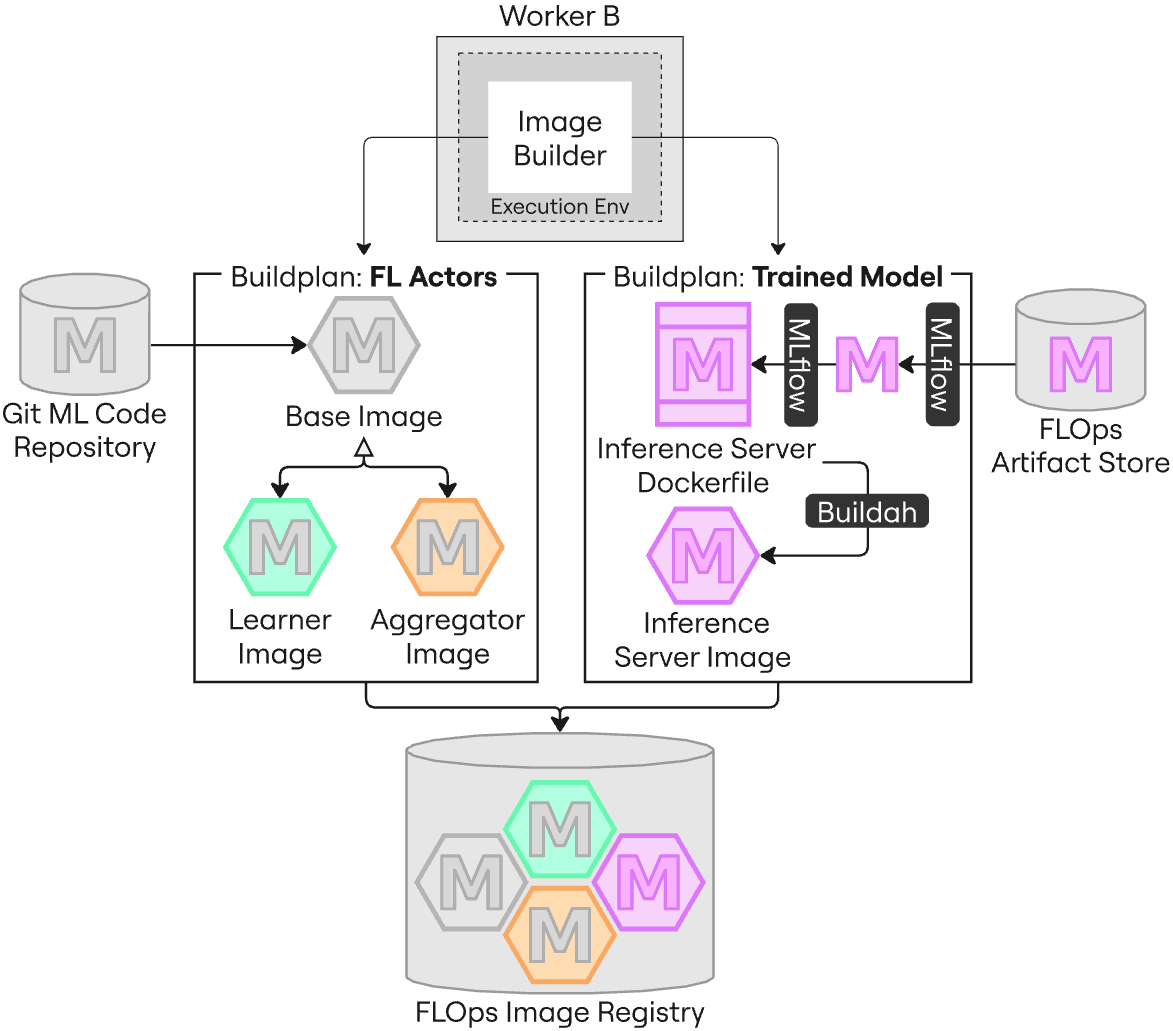
\includegraphics[width=0.80\paperwidth]{detailed_builder.png}
        \caption{Detailed FLOps Image Builder Processes}
        \label{fig:detailed_builder}
    \end{adjustwidth}
\end{figure}

Figure \ref{fig:detailed_builder} depicts the details how FLOps Image Builder works.
The grey Ms represent the untrained model (structure).
Purple Ms stand for the trained model.
Hexagons symbolize container images.
The service tracks the time different steps take and returns to the FLOps manager a summary of its total runtime and the runtime of individual steps.
The image builder supports two different build plans.

The first step in the FL Actors build plan is to fetch the user's ML code from his specified repository.
Secondly, the service builds a base image that contains all dependencies common to the learner and aggregator.
Due to the current multi-platform solution, the service pushes the base image to the image registry hosted in FLOps management.
Building and pushing the base image take up most of the service's total runtime.
The service continues to build the FL actor images one after another, pushing them in the end.
Thanks to the base image, these steps are relatively quick.
Pushing the base image does not generate meaningful overhead because of image layer caching.
The FL actor images reuse all the base image layers.
Thus, pushing them is accelerated, and the image registry recognizes and reuses its base image copy's layers.

Flower's design does not require the aggregator to possess any information about the model, including its structure or dependencies.
The aggregator's job is to average the received model parameters.
This process is based on simple mathematics and requires no other model-specific information or dependencies.
Therefore, the aggregator image and node can be relatively lightweight compared to the learners.
However, logging the trained model via MLflow requires access to the complete trained model, especially its structure.
The corresponding dependencies are necessary because a model structure is defined in a concrete ML framework.
Therefore, FLOps explicitly also includes these dependencies and the model structure in the aggregator.
During FL training only the model parameters are transmitted.
The aggregator's model copy is only needed at the very end of training.
The aggregator populates its untrained model copy via its final global model parameters.
This populated model gets logged.
Note that the model structure is initially defined in the user's ML repository and can be easily cloned and injected into images via the builder service.

The trained model build plan can only be run after the FL training is completed and the trained model is saved in the artifact store, which is hosted in the FLOps management.
MLflow provides commands to turn stored models into containers \cite{docs:mlfow_docker_cmds}.
The issue with this approach is that MLflow only provides this capability via Docker for all these commands, including building.
This approach works well directly on host machines but not inside containers (\ref{subsection:image_builders}).
As a workaround, FLOps uses MLflow to pull the stored trained model into the builder container.
Then, the service uses MLflow again to create a dockerfile based on this model.
FLOps' builder service augments this dockerfile to support multiple platforms and builds the trained model image via Buildah.
This built image wraps the trained model via an inference server.
One optional FLOps post-training step deploys this inference server directly after the builder service terminates.

\begin{figure}[b]
    \begin{changemargin}{0cm}{0cm}
        \centering
        \begin{tabular}{|c||c|c|c|c|c|c|}
            \hline
                \textbf{Image} & Image Builder & MLflow & Client & Server & SuperNode & SuperLink \\
            \hline
                \textbf{Size} & 3.0 GB & 819 MB & 1.16 GB & 1.13 GB & 232 MB & 232 MB
            \\
            \hline
        \end{tabular}
        \captionof{table}{Important FLOps Image Sizes (30.08.2024)} 
        \label{table:relevant_image_sizes_for_building}
    \end{changemargin}
\end{figure}

Table \ref{table:relevant_image_sizes_for_building} shows the sizes of different relevant images to provide more context for the final results and build processes.
The Image Builder image is the FLOps builder service.
It is noteworthy that FLOps' builder service without the MLflow (2.12.1) dependency is 900 MB and the official MLflow image is 819 MB.
The increase of more than 2.4 GB only due to this dependency is worth investigating.
The remaining images from the table are all from Flower \cite{flower_images}.
Flower recently introduced a significant change (Flower Next API \cite{docs:flower_next}) in how they use FL clients and servers.
They plan to deprecate the old approach that FLOps is using.
We tried migrating to the new Flower paradigm but encountered several issues with our current implementation.
Explaining Flower Next and FLOps' challenges with it would bloat this thesis.
This aspect is a great topic for future FLOps improvements.
The client and server images from the table are deprecated.
Their new replacements are the SuperNode and SuperLink, which are significantly smaller.
We mention these images to compare them with FLOps' FL actor images.

\begin{figure}[t]
    \begin{changemargin}{0cm}{0cm}
        \centering
        \begin{tabular}{|c|c|c|c|c|c|}
            \hline
                \textbf{Standalone} & \textbf{Base} & \textbf{Learner} & \textbf{Aggregator} & \textbf{Total Process} & \textbf{Base Image Build} \\
            \hline
                515 MB & 2.79 GB & 2.79 GB & 3.55 GB & 6min 20s & 3min 53s
            \\
            \hline
        \end{tabular}
        \captionof{table}{Simple Scikit-learn MNIST Build Example} 
        \label{table:sklearn_mnist_build_example}
    \end{changemargin}
\end{figure}
Table \ref{table:sklearn_mnist_build_example} shows a singular example of running a FLOps project using Scikit-learn and the MNIST dataset.
The Standalone refers to the standalone Scikit-learn image from Table \ref{table:ml_libs_images_compared}.
The base and learner images are equally large because the learner image only changes the files it works with but reuses all dependencies from the base image.
Therefore, the aggregator has a superset of the learner dependencies.
The total execution time for the builder service took 6 minutes and 20 seconds.
The base image build alone took almost four minutes.

FLOps Management uses and hosts an instance of the open-source CNCF (Cloud Native Computing Foundation) Distribution Registry \cite{docs:cncf_distribution_registry}.
This registry allows FLOps to be independent of any other registry provider.
FLOps has complete control and immediate access to this registry.


\subsection{Multi-Platform}

This subsection explains how FLOps builds multi-platform images.
Usually, end users build images only for a single platform.
Their builder knows their host's architecture and uses it as a target platform.
When inspecting popular public images, they support multiple target platforms.
Each image tag can have multiple digests, each representing a different platform.
For example, the latest Alpine image \cite{alpine_multiplatform_image} supports at least linux/amd64 and linux/arm/v6.
By default, it is impossible to run images that are intended for different architectures on machines with incompatible host architectures.
Specific workarounds via emulation exist.

The key of building and referencing images that support multiple platforms are manifests.
A plain manifest file contains information about a unique image digest.
This information includes its media type, size, layers, and architecture.
When an image supports multiple platforms, it has multiple digests, thus one manifest per digest.
Image indexes were invented to group these different manifests.
Note that image indexes refer to the OCI standard term \cite{oci_image_index}.
In Docker, they are called fat manifests or manifest lists \cite{docs:docker_manifest}.
As a result, different host architectures can use the same image tag and pull their matching digest image.
This happens because the local builder reads the image index and picks a suitable manifest.
Examples for manifests are available here \cite{docs:docker_manifest}.

Multi-platform images are a deep topic.
Because of its rapid development, many different media types, versions, and schemas for manifests exist.
Build machines need to use the same conventions as their image registries.
Discussing these details here would lead to bloat.
Excellent information about this topic is available here \cite{docs:image_manifest_versions_schemas}.

Previously, one had to manually build one image per target architecture on a machine of that architecture, provide the image tag with an architecture suffix, and push it.
Once all these different images were pushed, an image index had to be created and pushed.
Nowadays, a convenient solution for building multi-platform images is using docker's buildx builder \cite{docs:docker_buildx}.
It can build and push multi-platform images concurrently with a single command.

The FLOps image builder does not use docker to build its images (\ref{subsection:image_builders}).
Buildah also supports building multi-platform images but lacks the convenient new features of docker's buildx.
From our experience, Buildah lacks sufficient documentation regarding building and pushing multi-platform images.
We needed to look into its source code, read other sources, and experiment extensively until we made this work.

Another significant requirement for building multi-platform images on a single machine is emulating other architectures.
Otherwise, only images for the host's architecture can be built.
It is also possible to cross-compile or use multiple dedicated builder nodes with proper architectures \cite{docs:docker_multiplatform_image_builds}.
Conventionally, QEMU \cite{docs:quemu} is used to emulate such tasks.
Docker Desktop includes QEMU for Mac and Windows by default \cite{docs:docker_multiplatform_image_builds}.
QEMU translates the requested target architecture instructions into ones the host machine can understand.
Due to FLOps' special circumstances, which involve building complex images in orchestrated, containerd containers on heterogeneous devices, various approaches seem to be available to realize emulation.
Ideally, the emulator would be part of the builder image, thus avoiding the need to modify or require anything from the worker nodes.
After many unsuccessful attempts, we decided to require worker nodes that should build multi-platform images to pre-install QEMU.
For Linux machines, this can be done by installing an open-source package called qemu-user-static.

In conclusion, using this approach, the FLOps builder service can build multi-platform images.
All other FLOps (static) images, including the builder service or project observer, are also available for linux/amd64 and linux/arm64.
For example, all these images can be started on a Raspberry Pi 4, but these devices seem to lack sufficient resources to handle the FL training.
An additional downside of multi-platform image builds comes with the slowness of emulation.

Table \ref{table:sklearn_mnist_multi_platform_build_example} shows a simple example of FLOps' builder service's build times for different platforms.
The build machine natively supports linux/amd64.
Therefore, this build is much faster than the emulated arm one.
Both rows show the build times when only a single platform is requested.
The build times would be combined to support both platforms simultaneously.

\begin{figure}[t]
    \begin{changemargin}{0cm}{0cm}
        \centering
        \begin{tabular}{|c|c|c|c|c|c|c|}
            \hline
            \textbf{Builder Architecture} & \textbf{Target Platform} & \textbf{Full Build} & \textbf{Base Image} & \textbf{Actor Images} \\
            \hline
            linux/amd64 & linux/amd64 & 4min & 2min 30s & 1min 30s \\
            \hline
            linux/amd64 & linux/arm64 & 18min & 12min & 6min \\
            \hline
        \end{tabular}
        \captionof{table}{Simple Scikit-learn Multi-Platform Build Times Example} 
        \label{table:sklearn_mnist_multi_platform_build_example}
    \end{changemargin}
\end{figure}


